\documentclass[a4paper, 12pt]{report}

%%%%%%%%%%%%
% Packages %
%%%%%%%%%%%%

\usepackage[english]{babel}
\usepackage[noheader]{packages/sleek}
\usepackage{packages/sleek-title}
\usepackage{packages/sleek-theorems}
\usepackage{packages/sleek-listings}
\usepackage{xcolor}
\usepackage{cite}
\usepackage{graphicx}
\graphicspath{ {./images/} }

\definecolor{codegreen}{rgb}{0,0.6,0}
\definecolor{codegray}{rgb}{0.5,0.5,0.5}
\definecolor{codepurple}{rgb}{0.58,0,0.82}
\definecolor{backcolour}{rgb}{0.95,0.95,0.92}

\lstdefinestyle{mystyle}{
    backgroundcolor=\color{backcolour},   
    commentstyle=\color{codegreen},
    keywordstyle=\color{magenta},
    numberstyle=\tiny\color{codegray},
    stringstyle=\color{codepurple},
    basicstyle=\ttfamily\footnotesize,
    breakatwhitespace=false,         
    breaklines=true,                 
    captionpos=b,                    
    keepspaces=true,                 
    numbers=left,                    
    numbersep=5pt,                  
    showspaces=false,                
    showstringspaces=false,
    showtabs=false,                  
    tabsize=2
}

\lstset{style=mystyle}

%%%%%%%%%%%%%%
% Title-page %
%%%%%%%%%%%%%%

\logo{./images/hu_logo.jpeg}
\institute{Habib University}
\faculty{Dhanani School of Science and Engineering}
\department{CS412 Algorithms Design and Analysis}
\title{Shortest Path Problem}
\subtitle{Dr. Shah Jamal Alam}
\author{Muhammad Hammad Maqdoom \\ Alisha Momin \\ Fatima Nasir Khan \\ Lama Imam}
%\supervisor{Dr. Shah Jamal \textsc{Alam}}
\context{Project Report}
\date{Spring 2022}

%%%%%%%%%%%%%%%%
% Bibliography %
%%%%%%%%%%%%%%%%

% \addbibresource{./resources/bib/references.bib}

%%%%%%%%%%
% Others %
%%%%%%%%%%

\lstdefinestyle{latex}{
    language=TeX,
    style=default,
    %%%%%
    commentstyle=\ForestGreen,
    keywordstyle=\TrueBlue,
    stringstyle=\VeronicaPurple,
    emphstyle=\TrueBlue,
    %%%%%
    emph={LaTeX, usepackage, textit, textbf, textsc}
}

\FrameTBStyle{latex}

\def\tbs{\textbackslash}

%%%%%%%%%%%%
% Document %
%%%%%%%%%%%%

\begin{document}
    \maketitle
    \romantableofcontents
    \chapter{Introduction}
    \section{What is shortest path problem?}
	The shortest path problem is a graph theory problem that is mainly associated with finding the shortest path between two vertices or nodes in a graph that minimizes the total cost of traversing the graph or the sum of the weights of the edges traversed.\\
	\vspace{-0.9cm}
    \section{Cyclic and acylic graph}
    A cyclic graph is a graph containing at least one graph cycle. A graph that is not cyclic is said to be acyclic.\\
    \vspace{-0.9cm}
    \section{Directed and un-directed graph}
    A directed graph is a type of graph that contains ordered pairs of vertices while an undirected graph is a type of graph that contains unordered pairs of vertices.\\
    \vspace{-0.9cm}
    \section{Negative cycle and negative weighted cycle}
    A negative cycle is one in which the overall sum of the cycle becomes negative. Whereas a negative weight cycle is a cycle with weights that sum to a negative number. \\
    \vspace{-0.9cm}
    \section{Algorithms for determining the shortest path}
	\begin{itemize}
	\item Viterbi algorithm
    \item Dijkstra algorithm
    \item Bellman–Ford
    \item Johnson’s algorithm
    \item Floyd–Warshall algorithm
    \item A* search algorithm
    \end{itemize}
    The main focus of this report will be on BFS, Dijkstra, Bellman–Ford and Floyd- Warshall algorithm.
    
    \chapter{Algorithms}
    \section{Breath First Search (BFS)} 
	Breadth-first search is a graph traversal algorithm that starts traversing the graph from the root node and explores all the neighboring nodes. Then, it selects the nearest node and explores all the unexplored nodes. While using BFS for traversal, any node in the graph can be considered as the root node.\cite{BFS}
	
	BFS and its application in finding connected components of graphs were invented in 1945 by Konrad Zuse, in his (rejected) Ph.D. thesis on the Plankalkül programming language, but this was not published until 1972. It was reinvented in 1959 by Edward F. Moore, who used it to find the shortest path out of a maze, and later developed by C. Y. Lee into a wire routing algorithm (published 1961).\cite{BFS2}
	
	\subsection{Basic Intuition}
	Flowing steps are the basic intuition \cite{BFS1}
    \begin{enumerate}
        \item Choose any one node randomly, to start traversing.
        \item Visit its adjacent unvisited node.
        \item Mark it as visited in the boolean array and display it.
        \item Insert the visited node into the queue.
        \item If there is no adjacent node, remove the first node from the queue.
        \item Repeat the above steps until the queue is empty.
    \end{enumerate}
    
    \subsection{Algorithm}
    The pseudocode for BFS algorithm is given below:  \cite{BFS3}
    
    \begin{lstlisting}[language=Python]
    procedure BFS(G, root) is
        let Q be a queue
        label root as explored
        Q.enqueue(root)
        while Q is not empty do
            v := Q.dequeue()
                if v is the goal then
                    return v
                for all edges from v to w in G.adjacentEdges(v) do
                    if w is not labeled as explored then
                        label w as explored
                        Q.enqueue(w)
    \end{lstlisting}
The implementation to determine the time anaylsis is given below:
	\lstinputlisting[language=Octave]{BFS.py}
    \subsection{Complexity - Theoretical Analysis}
    The Time complexity of BFS is O(V + E) when Adjacency List is used and O(V$^2$) when Adjacency Matrix is used, where V stands for vertices and E stands for edges.
    
    \subsection{Assumptions and Limitations}
    BFS finds the shortest path in undirected and directed graph but it will not work on weighted graphs since the path with the fewest edges may not be the shortest if the edges it contains are expensive.
    
    \pagebreak
    \section{Dijkstra's Algorithm} 
	Dijkstra's algorithm is a method for determining the shortest paths between nodes in a graph, which can be used to represent, for instance, road networks. It was conceived in 1956 and published three years later by computer scientist Edsger W. Dijkstra. An SSSP (Single Source Shortest Path) algorithm is Dijkstra's algorithm. It determines the shortest route between any two points in the graph that is to determine the shortest path between a source node to all other nodes in the graph. The shortest path is determined using a greedy algorithm.
	
	\subsection{Basic Intuition}
	\begin{enumerate}
	    \item The Dijkstra algorithm is parameterized by the graph and the source vertex.
	    \item All nodes are initialized with a distance of "infinite" and the starting node (source node) is initialized with zero.
	    \item It makes a new priority queue that is empty. A tuple format is used to store each item in the queue that is (weight, vertex). In this, weight denotes the distance between the source and destination vertex.
	    \item The source vertex is placed in priority queue and distance is set to zero.
	    \item The priority queue will be iterated until it is empty.
	    \item It first obtain the vertex with the shortest distance from the priority queue within the loop, which we'll refer to as vertex u. After that it loops through all of u's adjacent vertices and performs the following for each adjacent vertex v. Vertex u's distance is updated if a shorter path to adjacent vertex v is found from vertex u. After that, it adds vertex v to the priority queue.
	\end{enumerate}
	
	\subsection{Algorithm}
	The pseudocode for Dijkstra algorithm is given below: \cite{Dijkstra} 
	
	\begin{lstlisting}[language=Python]
    function Dijkstra(Graph, source):
        # Initialization
        for each vertex v in Graph:    
            #initial distance from source to vertex v is set to infinite
            dist[v] := infinity 
            # Previous node in optimal path from source
            previous[v] := undefined  
        # Distance from source to source
        dist[source] := 0    
        # all nodes in the graph are unoptimized - thus are in Q
        Q := the set of all nodes in Graph 
        # main loop
        while Q is not empty:    
            u := node in Q with smallest dist[ ]
            remove u from Q
            # where v has not yet been removed from Q.
            for each neighbor v of u:    
                alt := dist[u] + dist_between(u, v)
                if alt < dist[v]    # Relax (u,v)
                    dist[v] := alt
                    previous[v] := u
        return previous[ ]
    \end{lstlisting}
    The implementation to determine the time anaylsis is given below:
	\lstinputlisting[language=Octave]{dijkstra.py}
	\subsection{Complexity - Theoretical Analysis}
	Dijkstra's Algorithm's theoretical complexity varies by data structure, the following are the theoretical complexities for each one:
	\begin{enumerate}
	    \item Priority queue and Adjacency list: \[O((V+E)*log(V))\]
	    \item Fibonacci Heap and adjacency list: 
	    \[O((E)+ V*log(V))\]
	    \item Priority queue and Matrix: \[O((V^2)+ E*log(V))\]
	\end{enumerate}
	
	\subsection{Assumptions and Limitations}
	The following are the necessary assumptions for implementing Dijkstra algorithm to solve the shortest-path problem for any weighted, directed graph with non-negative weights. It can handle graphs consisting of cycles but not graphs that consist of negative weighted cycles.
    
    \pagebreak
    \section{Bellman-Ford Algorithm} 
	The Bellman–Ford algorithm is an algorithm that computes shortest paths from a single source vertex to all of the other vertices in a weighted digraph. It is slower than Dijkstra's algorithm for the same problem, but more versatile, as it is capable of handling graphs in which some of the edge weights are negative numbers. The algorithm was first proposed by Alfonso Shimbel (1955), but is instead named after Richard Bellman and Lester Ford Jr., who published it in 1958 and 1956, respectively.
	
	\subsection{Basic Intuition}
	\begin{enumerate}
	    \item Initialize the distance for every vertex in the graph to infinite, the previous node's distance to null, and the source node's distance to 0.
	    \item Calculate a temporary distance for each vertex in the graph by adding the distance of the node and the edge's weight.
	    \item For nodes where the distance determined is less than the distance stored in the distance dictionary for such node, the distance is updated to the temporary distance and the previous distance is set to the new node in the distance dictionary.
	    \item If the distance between each edge (u,v) in the graph is less than the distance between the edges' weights, it indicates that the graph contains a negative cycle.
	\end{enumerate}
	
	\subsection{Algorithm}
	The pseudocode for Bellman-Ford algorithm is given below: \cite{Bellman-Ford} 
	\begin{lstlisting}[language=Python]
    function bellmanFord(G, S)
      for each vertex V in G
        distance[V] <- infinite
          previous[V] <- NULL
      distance[S] <- 0
    
      for each vertex V in G				
        for each edge (U,V) in G
          tempDistance <- distance[U] + edge_weight(U, V)
          if tempDistance < distance[V]
            distance[V] <- tempDistance
            previous[V] <- U
    
      for each edge (U,V) in G
        If distance[U] + edge_weight(U, V) < distance[V}
          Error: Negative Cycle Exists
    
      return distance[], previous[]
    \end{lstlisting}
    Our implementation to analyze the time is given below: 
    \lstinputlisting[language=Octave]{Bellman-ford.py}
	\subsection{Complexity - Theoretical Analysis}
	The Bellman-Ford algorithm is an algorithm that calculates the shortest paths in a weighted digraph from one source vertex to all other vertices. Bellman-Ford is also simpler than Dijkstra and suites well for distributed systems. But time complexity of Bellman-Ford is O(V*E), which is more than Dijkstra.
	
	\subsection{Assumptions and Limitations}
	Bellman-Ford does not work with undirected graph with negative edges as we end up with negative cycles that the Bellman Ford algorithm does not support.
	
	\pagebreak
	\section{Floyd–Warshall Algorithm} 
	Floyd-Warshall Algorithm is an algorithm for finding the shortest path between all the pairs of vertices in a weighted graph. This algorithm works for both the directed and undirected weighted graphs. But, it does not work for the graphs with negative cycles (where the sum of the edges in a cycle is negative). \\
	
	Floyd-Warhshall algorithm is also known as Floyd's algorithm, Roy-Floyd algorithm, Roy-Warshall algorithm, or WFI algorithm. This algorithm follows the dynamic programming approach to find the shortest paths.

	\subsection{Basic Intuition}
	\begin{enumerate}
	    \item Create a matrix $A^{0}$ of dimension n*n where n is the number of vertices. The row and the column are indexed as i and j respectively. i and j are the vertices of the graph. Each cell A[i][j] is filled with the distance from the $i^{th}$ vertex to the $j^{th}$ vertex. If there is no path from $i^{th}$ vertex to $j^{th}$ vertex, the cell is left as infinity.
	    \item Now, create a matrix $A^{1}$ using matrix $A^{0}$. The elements in the first column and the first row are left as they are. The remaining cells are filled in the following way.
	    
	    A[i][j] is filled with (A[i][k] + A[k][j]) if (A[i][j] $>$ A[i][k] + A[k][j])
	    
	    Let k be the intermediate vertex in the shortest path from source to destination. In this step, k is the first vertex. If the direct distance from the source to the destination is greater than the path through the vertex k, then the cell is filled with A[i][k] + A[k][j].
	    \item Similarly, $A^{2}$ is created using $A^{1}$. The elements in the second column and the second row are left as they are.
	    
	    In this step, k is the second vertex. The remaining steps are the same as in step 2.
	    \item Similarly, $A^{3}$ and $A^{4}$ is also created.
	    \item $A^{4}$ gives the shortest path between each pair of vertices.

	\end{enumerate}
	
	\subsection{Algorithm}
	The pseudocode for Floyd-Warshall algorithm is given below: 
	\begin{lstlisting}[language=Python]
    n = no of vertices
    A = matrix of dimension n*n
      for k = 1 to n
         for i = 1 to n
            for j = 1 to n
                Ak[i, j] = min (Ak-1[i, j], Ak-1[i, k] + Ak-1[k, j])
    return A
    \end{lstlisting}
The implementation to find the time is given below:
\lstinputlisting[language=Octave]{floyd-washall.py}
	\subsection{Complexity - Theoretical Analysis}
	The time Complexity of the Floyd-Warshall Algorithm is $O(n^3)$ or $O(|V|^3)$,such that V is the number of vertices or nodes in the graph. The run time has 3 as exponent because  there are three nested loops in the algorithm. This makes it less efficient than Bellman ford algorithm that has a run time of $O(|V|*|E|)$
	
	\subsection{Assumptions and Limitations}
	The Floyd-Warshall Algorithm is a weighted graph algorithm that finds the shortest path between all pairs of vertices. This approach works for weighted graphs that are both directed and undirected. It does not, however, operate for graphs with negative cycles (where the sum of the edges in a cycle is negative).
	
	\pagebreak
	\section{Fibonacci Heap Algorithm} 
    In computer science, a Fibonacci heap is a data structure for priority queue operations, consisting of a collection of heap-ordered trees. It has a better amortized running time than many other priority queue data structures including the binary heap and binomial heap. Michael L. Fredman and Robert E. Tarjan developed Fibonacci heaps in 1984 and published them in a scientific journal in 1987. Fibonacci heaps are named after the Fibonacci numbers, which are used in their running time analysis. Using Fibonacci heaps for priority queues improves the asymptotic running time of important algorithms, such as Dijkstra's algorithm for computing the shortest path between two nodes in a graph, compared to the same algorithm using other slower priority queue data structures.
	\cite{Fibonacci-Heap} 
	
	\subsection{Basic Intuition}
	Here is how Fibonacci heaps implement the basic functionalities of heaps and the time complexity of each operation.\\
	
	\textbf{Insert: }Insertion to a Fibonacci heap is similar to the insert operation of a binomial heap. A heap of one element is created and the two heaps are merged with the merge function. The minimum element pointer is updated if necessary. The total number of nodes in the tree increases by one.\\
	
	\textbf{Find Minimum: }The linked list has pointers and keeps track of the minimum node, so finding the minimum is simple and can be done in constant time.
	
	\textbf{Union: }Union of two Fibonacci heaps consists of following steps. Concatenate the roots of both the heaps. Update min by selecting a minimum key from the new root lists.\\
	
	\textbf{Extract Min: }It is the most important operation on a Fibonacci heap. In this operation, the node with minimum value is removed from the heap and the tree is re-adjusted. Deleting the minimum element is done in three steps. The node is removed from the root list and the node’s children are added to the root list. Next, the minimum element is updated if needed. Finally, consolidate the trees so that there are no repeated orders. If any consolidation occurred, make sure to update the minimum element if needed. Delaying consolidation saves times.
	\cite{Fibonacci-Heap2}
	
	\subsection{Algorithm}
	The algorithm is referred from \cite{Fibonacci-Heap2}
	\begin{lstlisting}[language = Python]
    Make-Fibonacci-Heap()
    n[H] := 0
    min[H] := NIL 
    return H
    
    Fibonacci-Heap-Minimum(H)
    return min[H]
    
    Fibonacci-Heap-Link(H,y,x)
    remove y from the root list of H
    make y a child of x
    degree[x] := degree[x] + 1
    mark[y] := FALSE
    
    CONSOLIDATE(H)
    for i:=0 to D(n[H])
         Do A[i] := NIL
    for each node w in the root list of H
        do x:= w
           d:= degree[x]
           while A[d] <> NIL
               do y:=A[d]
                  if key[x]>key[y]
                    then exchange x<->y
                  Fibonacci-Heap-Link(H, y, x)
                  A[d]:=NIL
                 d:=d+1
           A[d]:=x
    min[H]:=NIL
    for i:=0 to D(n[H])
        do if A[i]<> NIL
              then add A[i] to the root list of H
                   if min[H] = NIL or key[A[i]]<key[min[H]]
                      then min[H]:= A[i]
    
    Fibonacci-Heap-Union(H1,H2)
    H := Make-Fibonacci-Heap()
    min[H] := min[H1]
    Concatenate the root list of H2 with the root list of H
    if (min[H1] = NIL) or (min[H2] <> NIL and min[H2] < min[H1])
       then min[H] := min[H2]
    n[H] := n[H1] + n[H2]
    free the objects H1 and H2
    return H
    
    
    Fibonacci-Heap-Insert(H,x)
    degree[x] := 0
    p[x] := NIL
    child[x] := NIL
    left[x] := x
    right[x] := x
    mark[x] := FALSE
    concatenate the root list containing x with root list H
    if min[H] = NIL or key[x]<key[min[H]]
            then min[H] := x
    n[H]:= n[H]+1
    
    Fibonacci-Heap-Extract-Min(H)
    z:= min[H]
    if x <> NIL
            then for each child x of z
                 do add x to the root list of H
                    p[x]:= NIL
                 remove z from the root list of H
                 if z = right[z]
                    then min[H]:=NIL
                    else min[H]:=right[z]
                         CONSOLIDATE(H)
                 n[H] := n[H]-1
    return z
    
    Fibonacci-Heap-Decrease-Key(H,x,k)
    if k > key[x]
       then error "new key is greater than current key"
    key[x] := k
    y := p[x]
    if y <> NIL and key[x]<key[y]
       then CUT(H, x, y)
            CASCADING-CUT(H,y)    
    if key[x]<key[min[H]]
       then min[H] := x
    
    CUT(H,x,y)
    Remove x from the child list of y, decrementing degree[y]
    Add x to the root list of H
    p[x]:= NIL
    mark[x]:= FALSE
    
    CASCADING-CUT(H,y)
    z:= p[y]
    if z <> NIL
      then if mark[y] = FALSE
           then mark[y]:= TRUE
           else CUT(H, y, z)
                CASCADING-CUT(H, z)
    
    Fibonacci-Heap-Delete(H,x)
    Fibonacci-Heap-Decrease-Key(H,x,-infinity)
    Fibonacci-Heap-Extract-Min(H)
	\end{lstlisting}
	My implementation to analyze the time is given below:\\
	In import fibonnaciheap, we have used the below code:
	\lstinputlisting[language=Octave]{fibonnaciheap.py}
	The main file is given below:
	\lstinputlisting[language=Octave]{fib-dijskra.py}
	\subsection{Complexity - Theoretical Analysis}
	The time complexity of Fibonacci heap is given below: 
	\begin{center}
	    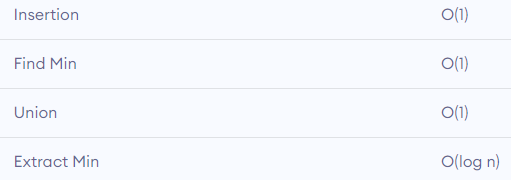
\includegraphics[width=12cm]{images/fibonacci-Heap.PNG}
	\end{center}
	
	\subsection{Assumptions and Limitations}
	Fibonacci heaps have a reputation for being slow in practice due to large memory consumption per node and high constant factors on all operations. Recent experimental results suggest that Fibonacci heaps are more efficient in practice than most of its later derivatives, including quake heaps, violation heaps, strict Fibonacci heaps, rank pairing heaps, but less efficient than either pairing heaps or array-based heaps.
	
	\chapter{Empirical Analysis}
    
    To implement BFS we used an adjacency matrix approach and monitored their performance on graphs with varying numbers of nodes to determine their time complexity.\\
    \\
    With regards to the implementations of Dijkstra and Bellman Ford we created graphs in Python using the Numpy library and generated random n by n matrices using the Numpy random built-in function that is numpy.random.randint(range of value, size of matrix). We assumed that all of these randomly generated values were positive in order to ensure compatibility with Dijkstra and Bellman-Ford algorithms and the absence of negative cycles. We used Python's native time library to record the time it took for Dijkstra and Bellman Fords algorithms to find the shortest path from the selected node to all other nodes in the graphs. We displayed these data and analyzed the time complexities by comparing the empirical value to theoretical values by plotting the results for a range of node counts, n, from 25 to 5000.\\
    \\
    For Floyd-Warshall we created an adjacency matrix whose size gradually increased through increasing the number of nodes. The matrix was initialized with non-negative weights that were attached to each edge. Using present libraries we run and executed the algorithm and represent the run time and number of nodes on the graph to analyze time complexity and compare theoretical and empirical values. \\
    
    
    \begin{figure}
          \centering
          \includegraphics[width=12cm]{images/BFS.png}
          \caption{\textbf{Graph of BFS Algorithm time analysis}}   
          \label{fig:picture1}
    \end{figure} 
    \begin{figure}
          \centering
          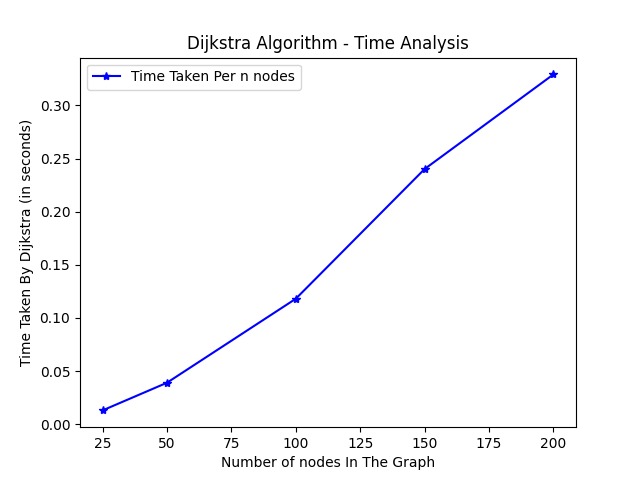
\includegraphics[width=12cm]{images/dijkstra2.png}
          \caption{\textbf{Graph of Dijkstra Algorithm time analysis}}   
          \label{fig:picture2}
    \end{figure} 
    \begin{figure}
          \centering
          \includegraphics[width=12cm]{images/dijsktra-n=5k.png}
          \caption{\textbf{Graph of Dijkstra Algorithm time analysis}}   
          \label{fig:picture3}
    \end{figure} 
    
    \begin{figure}
          \centering
          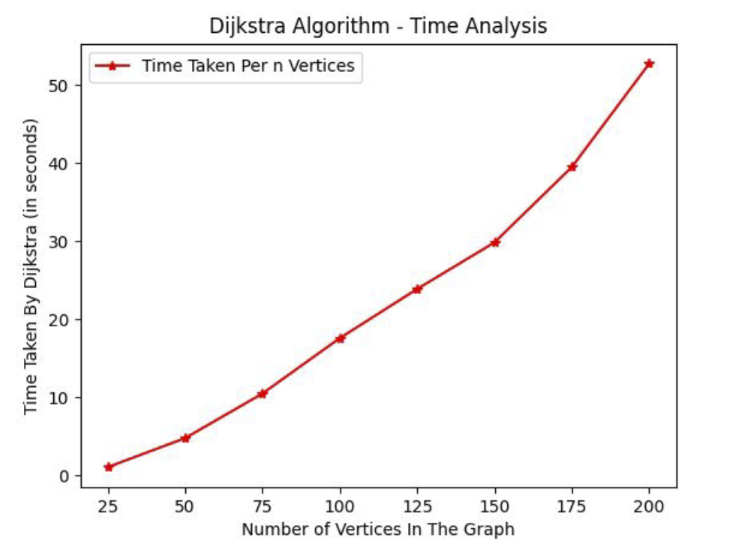
\includegraphics[width=12cm]{images/fibheapdj.png}
          \caption{\textbf{Graph of Dijkstra Algorithm using Fibonacci Heap time analysis}}   
          \label{fig:picture4}
    \end{figure}      
    \begin{figure}      
          \centering
          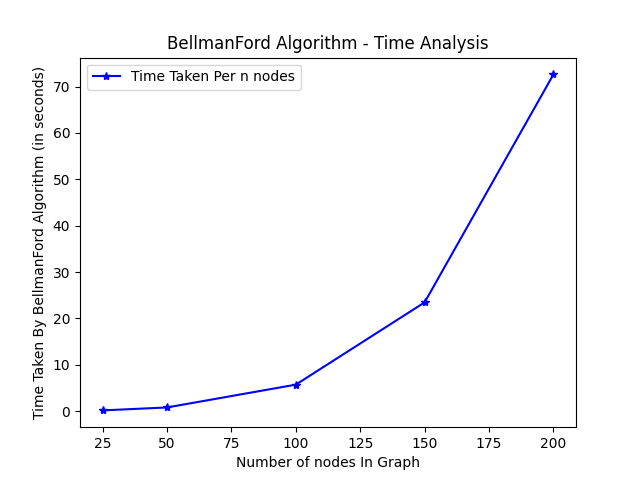
\includegraphics[width=12cm]{images/bellman-ford.png}
          \caption{\textbf{Graph of Bellman-Ford Algorithm time analysis}}   
          \label{fig:picture5}
    \end{figure}
    \begin{figure}
        \centering
        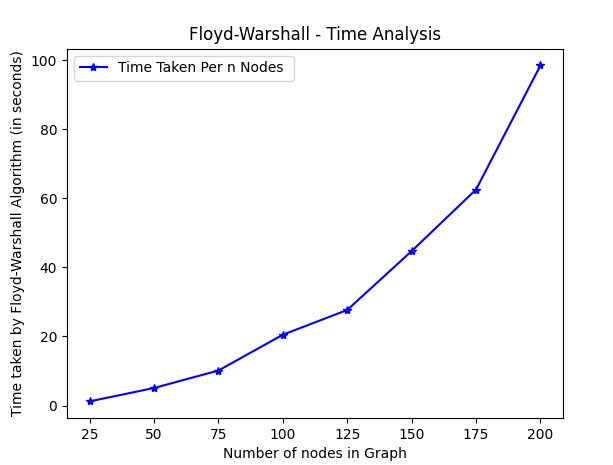
\includegraphics[width=12cm]{images/Floyd-Warshall.JPG}
        \caption{Graph of Floyd-Warshall Algorithm time analysis}
        \label{fig:picture6}
    \end{figure}
    \begin{figure}
        \centering
        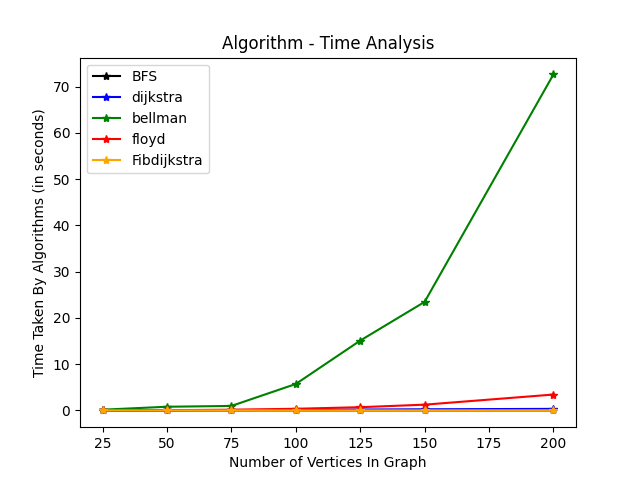
\includegraphics[width=12cm]{images/comparision.png}
        \caption{Comparison of all Algorithm time analysis}
        \label{fig:picture7}
    \end{figure}
    
    \pagebreak
    \section{Results}

    BFS calculates the shortest paths in unweighted graphs.On the other hand, Dijkstra's algorithm calculates the same thing in weighted graphs.BFS runs in O(E+V), while Dijkstra's runs in O((V+E)*log(V)). As is clear from the performance graphs above, Djikistra performs significantly better than BFS.\\

    We discovered that Dijkstra performed flawlessly in our empirical time analysis, taking roughly linear time to identify the shortest path between n nodes, as depicted in the graph.\\
    
    We achieved a nearly quadratic graph for Bellman Ford's Algorithm due to the constraints we imposed on our input matrices, that insured that each of nodes was linked to at least single edge, implying that the edges number E is at least V+1. Thus, we can say that this graph empirically satisfies our theoretical complexity because our theoretical complexity has been reduced from O(V*E) to O(V$^2$).\\
    
    The Floyd-Warshall algorithm comes close to $O(V^3)$ in the practical model. The matrice has no negative weighted edges and they are randomly assigned.\\
    
    Hence we conclude that Dijkstra algorithm is significantly much better than Bellman-Ford algorithm with regards to time complexity. Although, Dijkstra algorithm doesn't work for negative weighted graphs therefore we use Bellman-Ford algorithm to efficiently perform the computation for negative weighted graphs. The Bellman ford algorithm is much better in terms of run time as compared with Floyd-Warshall algorithm. Floyd-Warshall works with undirected unlike Bellman Ford, thus it is used for undirected graphs over Bellman Ford despite Bellman Ford having a better runtime.\\
    
    Additionally we implemented a priority queue and compared Djikstra's performance. Dijkstra's original shortest path algorithm does not use a priority queue, and runs in $O(V^{2})$ time. When using a Fibonacci heap as a priority queue, it runs in O(E + V log V) time, which is asymptotically the fastest known time complexity for this problem. However, due to their programming complexity, and for some practical purposes, Fibonacci heaps are not always a necessary or significant improvement. This is evident by the runtime graphs plotted below for both implementations.\\
    
    We finally plotted the run time graphs of all the algorithms chosen for our project to be able to analyse and compare their overall trends As we can see in figure 3.7 Dijkstra and BFS have completely overlapping lines indicating how close in performance they are but Dijkstra is significantly better than BFS according to our time complexity analysis. \\
    
    Next we see Dijkstra’s implementation with a Fibonacci heap falls just above Dijkstra’s performance indicating that despite it having the fastest asymptotic  time complexity it doesn’t cause significant improvement in the shortest path problem. \\
    
    Floyd Warshall on the other hand takes a much longer time than Dijkstra and BFS and Fibonacci heap combined. Bellman ford takes even longer than Floyd Warshall in solving the shortest path problem.\\
    \pagebreak
    
    \section{Limitations}
    
    For our empirical analysis we tried to vary our number of vertices in the graph as greater than 200. But due to machine limitations we were unable to execute any number greater than 200.\\
    \pagebreak
    
    
    \chapter{Theoretical Comparison}
    
BFS finds the shortest path in undirected and directed graph but it will not work on
weighted graphs since the path with the fewest edges may not be the shortest if the 
edges it contains are expensive. The Time complexity of BFS is O(V + E) when Adjacency 
List is used and O($V^2$) when Adjacency Matrix is used.
\\
    
To deal with this limitation Djikstra comes in. The main advantage of Dijkstra’s algorithm is its considerably low complexity, an almost linear complexity. It works correctly for directed and un-directed graphs, however, when working with negative weights, Dijkstra’s algorithm can’t be used. Also, when working with dense graphs, where E is close to $V^2$, if we need to calculate the shortest path between any pair of nodes, using Dijkstra’s algorithm is not a good option as the complexity will then be O($V^2$ log(V)).
\\

The main advantage of the Bellman-Ford algorithm is its capability to handle negative weights in addition to directed and un-directed graphs. However, the Bellman-Ford algorithm has a considerably larger complexity than Dijkstra’s algorithm. Therefore,
Dijkstra’s algorithm has more applications, because graphs with negative weights are usually considered a rare case. As mentioned earlier, the Bellman-Ford algorithm can handle directed and directed graphs with negative weights. However, it can only handle directed graphs with negative weights, as long as we don’t have negative cycles. To avoid this limitation we come to the Floyd-Warshall.\\

Floyd-Warshall Algorithm is an algorithm for finding the shortest path between all the pairs of vertices in a weighted graph. This algorithm works for both the directed and undirected weighted graphs. But, it does not work for the graphs with negative cycles.\\
    
    \chapter{Task Distribution}
    \begin{itemize}
        \item Muhammad Hammad Maqdoom worked on BFS\\
        \item Alisha Momin worked on Dijkstra And Bellman Ford\\
        \item Lama Imam and Fatima Nasir Khan worked on Floyd Warshall and Fibonacci heap for Dijkstra\\ 
        \item Lama Imam and Fatima Nasir Khan worked on the presentation and poster for Demo\\
    \end{itemize}
    
    \pagebreak
    \begin{thebibliography}{9}
    
    \bibitem{BFS1}
    \url{https://techvidvan.com/tutorials/breadth-first-search/#:~:text=Algorithm\%20for\%20BFS\%3A,visited\%20node\%20into\%20the\%20queue.}
    
    \bibitem{BFS3}
    \url{https://en.wikipedia.org/wiki/Breadth-first_search} 
    
    \bibitem{Dijkstra}
    \url{http://www.gitta.info/Accessibiliti/en/html/Dijkstra_learningObject1.html}
    
    \bibitem{Bellman-Ford}
    \url{https://www.programiz.com/dsa/bellman-ford-algorithm}
    
    \bibitem{BFS}
    \url{https://www.javatpoint.com/breadth-first-search-algorithm}
    
    \bibitem{BFS2}
    \url{https://en.wikipedia.org/wiki/Breadth-first_search}
    
    \bibitem{Floyd-Warshall}
    \url{https://www.programiz.com/dsa/floyd-warshall-algorithm}
    
    \bibitem{Fibonacci-Heap}
    \url{https://en.wikipedia.org/wiki/Fibonacci_heap}
    
    \bibitem{Fibonacci-Heap2}
    \url{https://brilliant.org/wiki/fibonacci-heap/}
    
    \bibitem{Fibonacci-Heap3}
    \url{https://kbaile03.github.io/projects/fibo_dijk/fibo_dijk.html}
    \bibitem{Fibonacci-Heap4}
    \url{https://www.programiz.com/dsa/fibonacci-heap}
    \end{thebibliography}
       
   



\end{document}
